\section{Brüche}\label{sec:Brueche}
Brüche sind in der Mathematik grundlegenden für das Verständnis für viele Rechnungen. Dabei sind sie oftmals genauer als Dezimalbrüche, da sie, im Gegenteil zu Dezimalbrüchen, periodische Zahlen darstellen können, ohne sie Runden zu müssen. Dies bedeutet Brüche sind deutlich genauer im Vergleich zu Dezimalbrüchen. Dabei ist ein Bruch nicht anders als eine andere Darstellungsweise für eine Division.
\subsection{Termination}\label{sec:Brueche/Termination}
 Bezüglich der Termination von Brüchen gilt Folgendes.\\
\[\color{red}a:\color{blue}b\color{black}= \frac{\color{red}a}{\color{blue}b}\]
Wobei $\color{red}{a}$ bei einem Bruch als Zähler bezeichnet wird und dabei angibt, wie viele Bruchteile des Nenners gegeben sind.  $\color{blue}{b}$ ist hierbei der Nenner und bestimmt den Namen des Bruches.
\subsection{Erweitern und kürzen von Brüchen}\label{sec:Brueche/Erweitern und kuerzen von Bruechen}
In manchen Situationen ist es notwendig, den Namen eines Bruches zu verändern, aber seinen Wert beizubehalten. Hierbei liegt das Prinzip eines Verhältnisses zugrunde. So stellt ein Bruch $\frac{1}{2}$ den gleichen Sachverhalt dar, wie der Bruch $\frac{4}{8}$.
\subsubsection{Erweitern von Brüchen} Durch das Multiplizieren von Zähler und Nenner in einem Bruch mit einer Zahl wird der ursprüngliche Bruch erweitert. 
\begin{paracol}{2}
	\begin{flushleft}
	\begin{beispiel}
\[\overset{\cdot3}{\overrightarrow{\frac{\color{red}6}{7}=\frac{\color{red}18}{21}}}\]
	\end{beispiel}
	\end{flushleft}	
\switchcolumn
	\begin{flushright}
		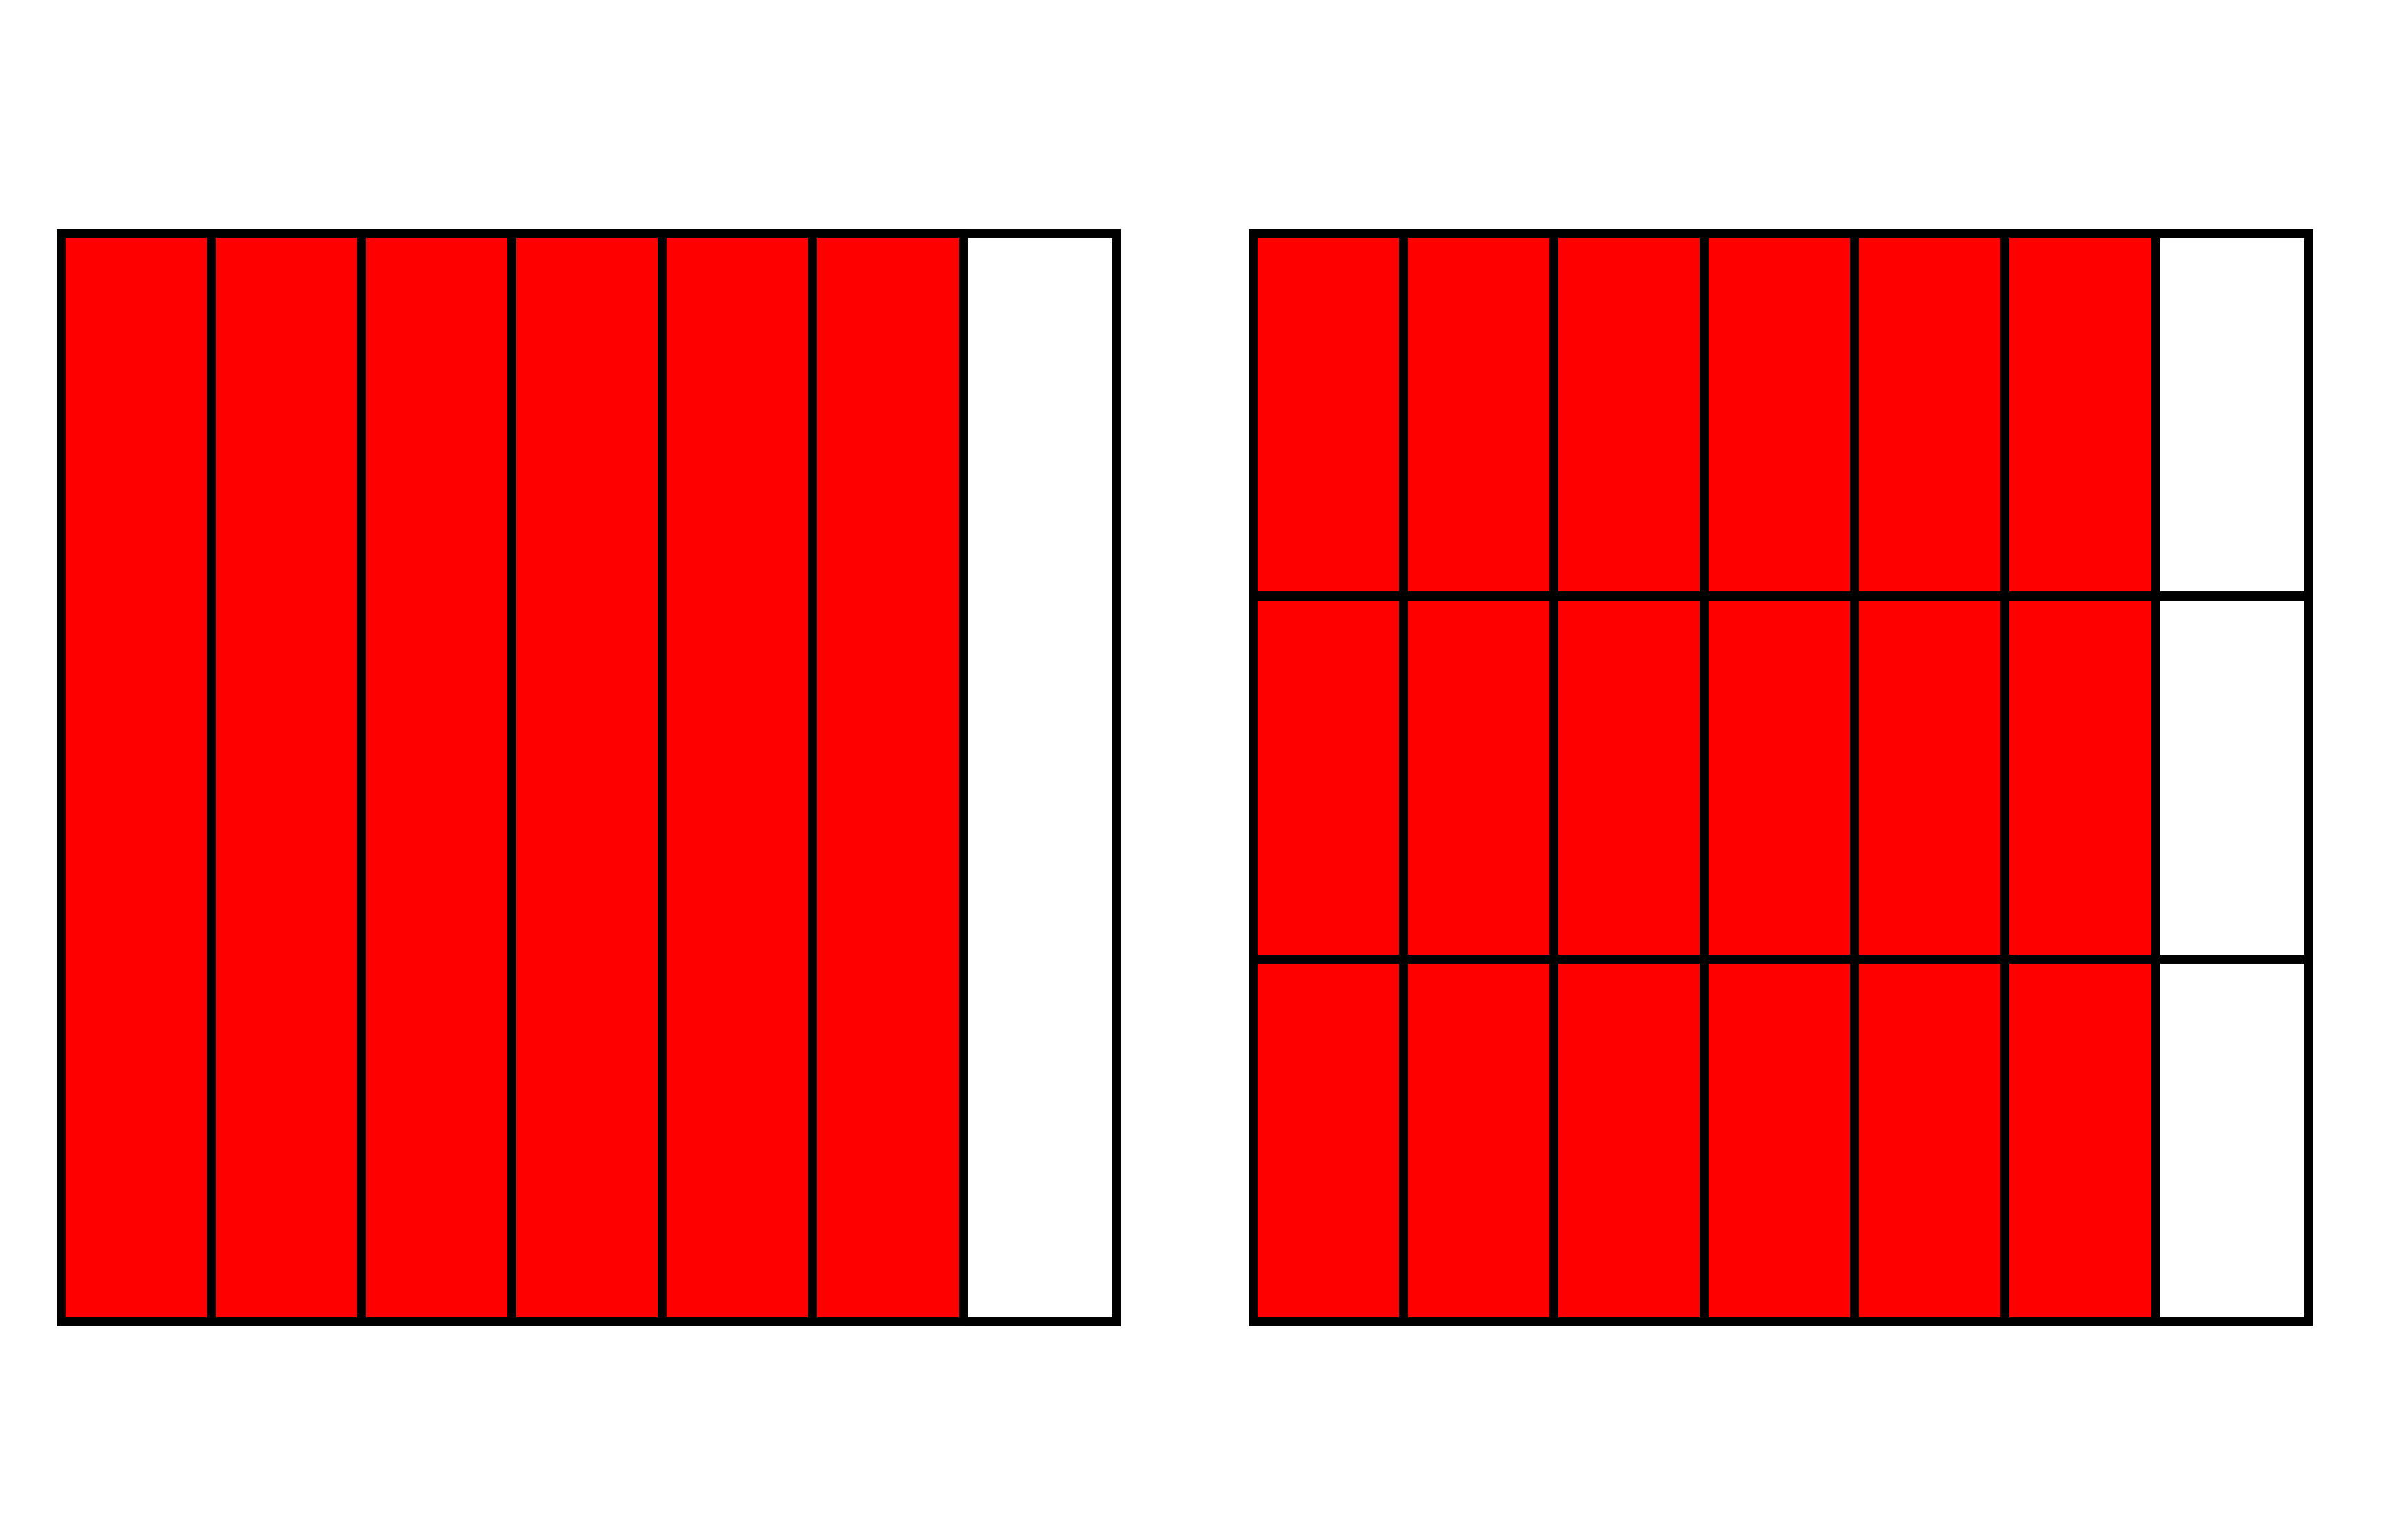
\includegraphics[width=5cm]{Media/Theorieheft-Brueche-Erweitern.png}
	\end{flushright}
\end{paracol}
\subsubsection{Kürzen von Brüchen}
Das Kürzen von Brüchen funktioniert ähnlich wie beim Erweitern, bloß umgedreht.

\begin{beispiel}
	\[\frac{\color{red}8}{28}=\frac{\color{red}2}{7}\]
\end{beispiel}

\subsubsection{Faktorisieren} Da beim Rechnen mit Brüchen ebenfalls alle Rechengesetzte gelten, kann man im Zähler und im Nenner faktorisieren.

\begin{beispiel}
	\[\frac{5x-5}{10x-5}=\frac{5\cdot(x-1)}{5\cdot(2x-1)}=\frac{x-1}{2x-1}\]
\end{beispiel}
\subsection{Rechnen mit Brüchen}\label{sec:Brueche/Rechen mit Bruechen}
Da auch mit Brüchen in der Mathematik gerechnet wird, gelten auch die Grundrechenarten.
\subsubsection{Addition und Subtraktion} Beim addieren und subtrahieren von Brüchen, muss darauf geachtet werden, dass beide Brüche gleichnamig sin. 

\begin{beispiel}
	\begin{align*}
		&\frac{2}{7}+\frac{3}{12}\\
		&=\frac{2}{7}+\frac{3}{12}\\
		&= \frac{24}{84}+\frac{21}{84}\\
		&= \frac{45}{84}
	\end{align*}	
\end{beispiel}
\subsubsection{Multiplizieren} Das Multiplizieren von Brüchen ist weniger aufwendig im Vergleich zu der Subtraktion und Addition, denn bei der Multiplikation wird lediglich der Nenner mit dem Nenner und der Zähler mit dem Zähler multipliziert.

\begin{beispiel}
	\[\frac{3}{4}\cdot\frac{7}{2}=\frac{21}{8}\]
\end{beispiel}
\subsubsection{Division} Bei der Division von Brüchen nimmt man lediglich den Kehrbruch des zu dividierenden Bruch und multipliziert ihn mit dem ersten Bruch. 

\begin{beispiel}
	\[\frac{3}{4}:\frac{4}{7} \rightarrow \frac{3}{4}\cdot \frac{7}{4}= \frac{21}{12}\]
\end{beispiel}